\documentclass[languages_and_machines.tex]{subfiles}
\begin{document}

\begin{frame}
  \frametitle{Goals}
  \begin{enumerate}
  \item Give you an overview of language classes and machine types
  \item Don't just think about computable/non-computable; Think about computable \textit{with what}
  \item Subsets of Turing Complete; next week, supersets
  \end{enumerate}
\end{frame}

\begin{frame}

  \frametitle{Mathy Definitions}

  \textbf{Concatenation} \pause \(a(bc) = abc = (ab)c\)\pause, \(\varepsilon a = a = a \varepsilon\)

  \pause

  \textbf{Concatenation of sets} \(\Sigma \Gamma := \{\sigma \gamma : \sigma \in \Sigma, \gamma \in \Gamma\}\)

  \pause

  \textbf{Kleene star} \(\Sigma^* := \{\varepsilon\} \cup \Sigma \cup \Sigma^2 \cup \dotsb\) \\
  where \(\Sigma^2 = \Sigma \Sigma\) (Star means arbitrary repetitions)

  \pause

  \textbf{Language over alphabet \(\Sigma\)} := subset of \(\Sigma^*\)
  \\ The strings are considered `valid words' of the language.

\end{frame}

\begin{frame}
  \frametitle{Definitions}

  \textbf{Formal Grammar} :=

\begin{itemize}
  \item finite set of terminals (convention: lowercase)
  \item finite set of nonterminals (convention: uppercase)
  \item start symbol (convention: S)
  \item finite set of rules (pair of strings)
  \end{itemize}
  
Grammars generate languages.

  \textbf{Abstract Machine} := ?
  \\ Machines can decide if a string is in a language.

\end{frame}

\begin{frame}
  \frametitle{Grammar semantics}

  \begin{itemize}
  \item G := (a-z, A-Z, S, the following rules)
    \begin{enumerate}
    \item S \pro aSb
    \item S \pro \emptystr
    \end{enumerate}
    \pause

  \item S \pause \pro aSb \pause \pro aaSbb \pause \pro aaaSbbb \pause \pro aaabbb
    \pause

  \item The language generated by \(G\) is \pause \(\{a^nb^n | n \in \mathbb N\}\).
  \end{itemize}
\end{frame}

\begin{frame}
  \frametitle{Lindenmayer system}

  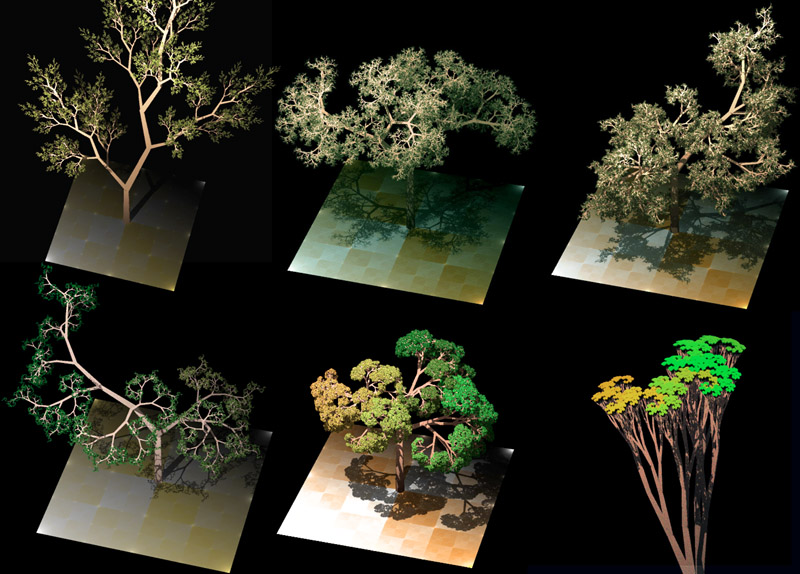
\includegraphics[width=1\textwidth]{L-system-1.jpg}
\end{frame}

\begin{frame}
  \frametitle{Lindenmayer system}

  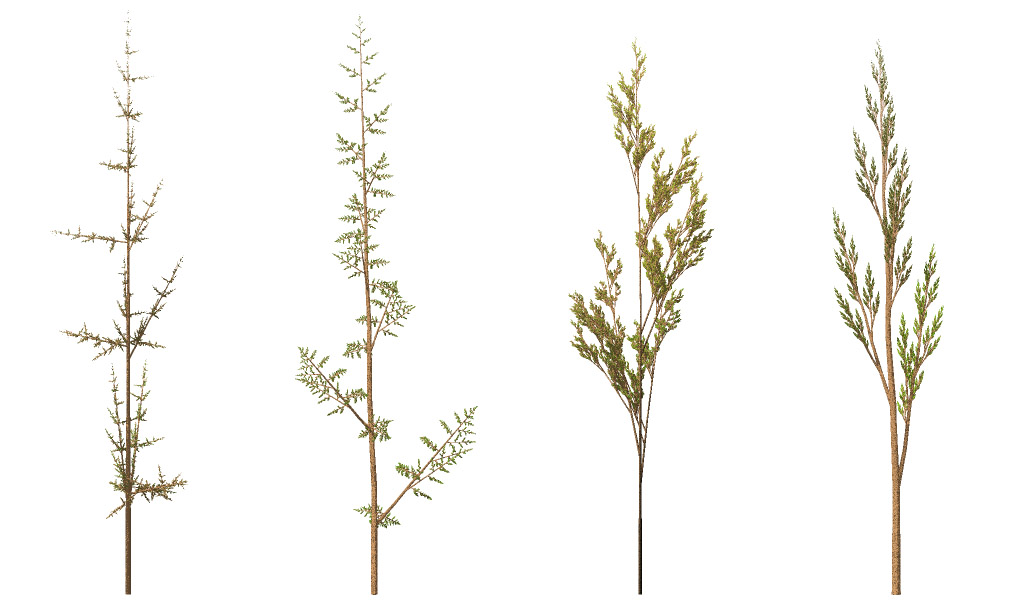
\includegraphics[width=1\textwidth]{L-system-2.jpg}
\end{frame}

\begin{frame}
  \frametitle{Grammar \(\iff\) machine}

  \textit{Grammar generates} string in the language

  \textit{Machine recognizes} a string that is in the language
\end{frame}

\begin{frame}
  \frametitle{Language relates to computing}

  \begin{itemize}
  \item Consider language \(L\) consisting of factorials \(\{\)``1'', ``1'', ``2'', ``6'', ``24'', \ldots \(\}\)
    \pause
  \item A generator/recognizer would have to compute the factorial.
  \end{itemize}
\end{frame}

\begin{frame}
  \frametitle{Language hierarchy}

 simple languages, quick machines \(\rightleftharpoons\) complex languages, slow machines

  \vspace{7mm}
  \pause

  Chomsky Hierarchy (1956):

  % 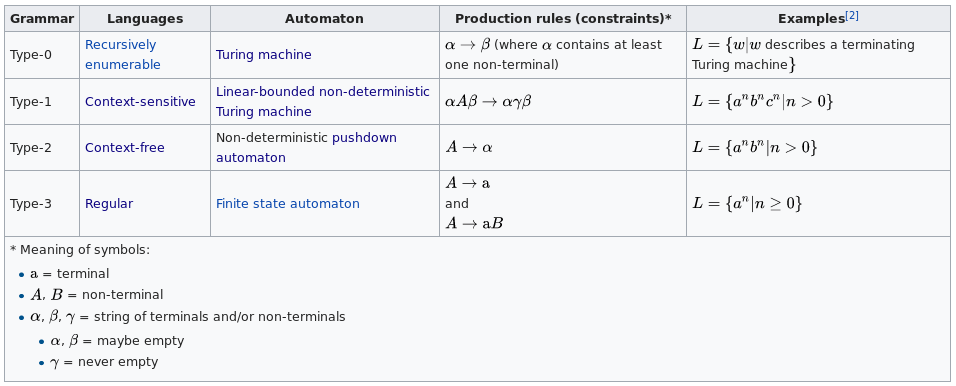
\includegraphics[width=\textwidth]{chomsky_table.png}

  {\footnotesize
  \begin{tabular}{l||l|p{5cm}}
    Language class & Grammar & Type of machine
    \\ \hline \hline Regular & A \pro Yz & deterministic finite-state automata
    \\ \hline Context-free & A \pro \(\gamma\) & deterministic pushdown automata
    \\ \hline Context-sensitive & \(\alpha \mathrm{A} \beta\) \pro \(\alpha \gamma \beta\) & linear-bounded non-deterministic Turing machine
    \\ \hline Recursively Enumerable & \(\alpha\) \pro \(\beta\) & Turing machine
    % \\ \hline Inomputable & none & none
                                     % TODO: should there be a class of languages that there is no grammar for? Perhaps the language of programs that halt? Perhaps not, because even thse would be recursively enumerable, just not recursive.
    \\
  \end{tabular}

  where \(\alpha, \beta, \gamma\): strings of terminals and non-terminals \\
  }
\end{frame}

\begin{frame}
  \frametitle{Language hierarchy}

  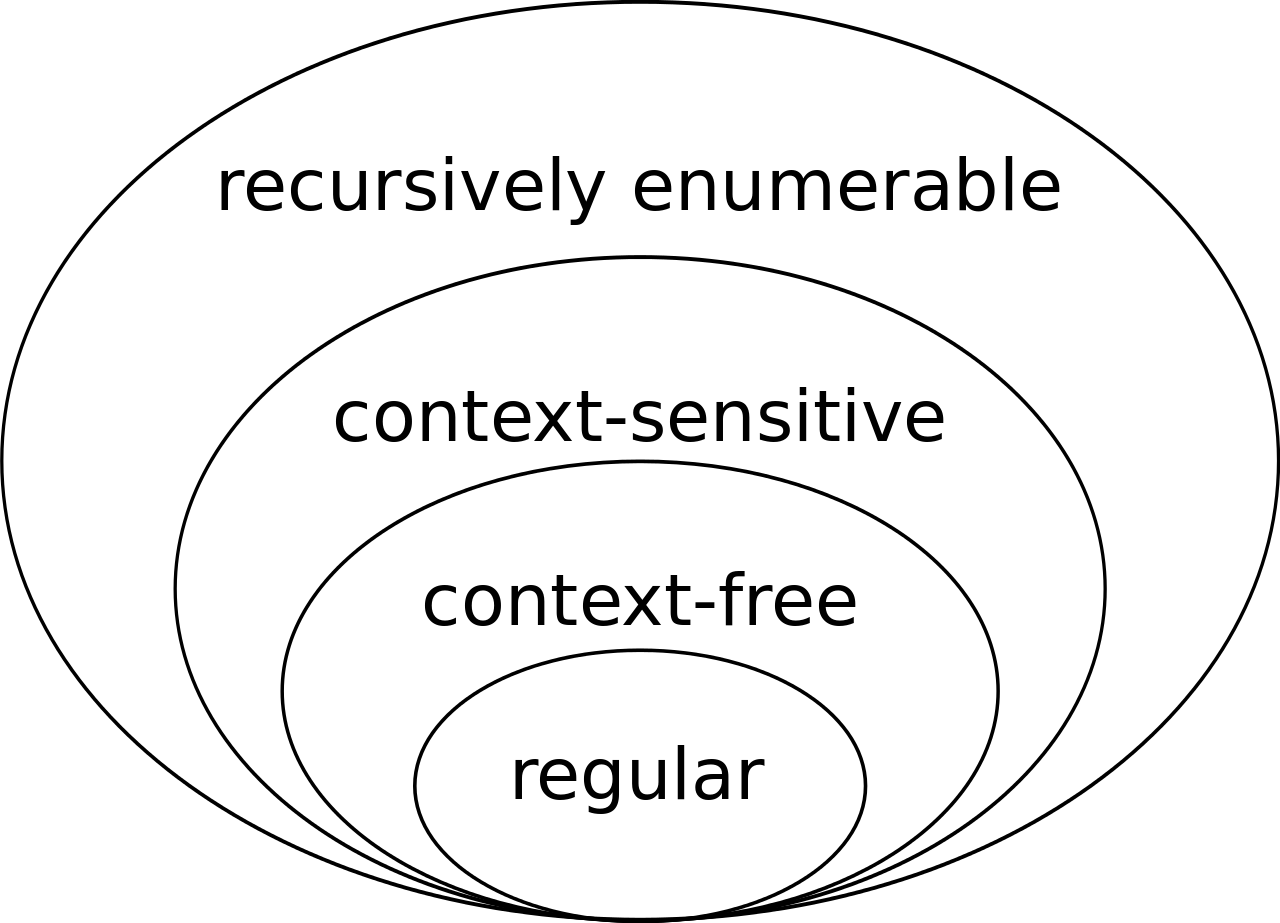
\includegraphics[width=0.9\textwidth]{chomsky-chart.png}

  {\tiny
    Figure from \href{https://commons.wikimedia.org/wiki/File:Chomsky-hierarchy.svg}{WikiMedia}
  }

\end{frame}

\end{document}

%%% Local Variables:
%%% mode: latex
%%% TeX-master: t
%%% End:
